\documentclass[master=cws,masteroption=gs]{kulemt}

\setup{title={Automatisch uitrol van database systemen en vergelijking van beschikbaarheid},
  author={Thomas Uyttendaele},
  promotor={Prof.\,dr.\,ir.\ Wouter Joosen},
  assessor={Ir.},
  assistant={Ir.\ B. Vanbrabant}}
% De volgende \setup mag verwijderd worden als geen fiche gewenst is.
\setup{filingcard,
  translatedtitle={Automatisch uitrol van database systemen en vergelijking van beschikbaarheid},
  udc=681.3,
  shortabstract={Hier komt een heel bondig abstract van hooguit 500
      woorden. \LaTeX\ commando's mogen hier gebruikt worden. Blanco lijnen
   (of het commando \texttt{\string\pa r}) zijn wel niet
   toegelaten!
  \endgraf \lipsum[2]}}
% Verwijder de "%" op de volgende lijn als je de kaft wil afdrukken
%\setup{coverpageonly}
% Verwijder de "%" op de volgende lijn als je enkel de eerste pagina's wil
% afdrukken en de rest bv. via Word aanmaken.
%\setup{frontpagesonly}

% Kies de fonts voor de gewone tekst, bv. Latin Modern
\setup{font=lm}

% Hier kun je dan nog andere pakketten laden of eigen definities voorzien

% Tenslotte wordt hyperref gebruikt voor pdf bestanden.
% Dit mag verwijderd worden voor de af te drukken versie.
\usepackage[pdfusetitle,colorlinks,plainpages=false]{hyperref}
\usepackage[dutch]{babel}
\usepackage{lipsum} % for dummy text only
\usepackage{todonotes}
\usepackage{csquotes}
\usepackage[backend=bibtex]{biblatex}
\usepackage[acronym]{glossaries}
\usepackage{eurosym}
\usepackage{subfigure}
\usepackage{tikz}
\usetikzlibrary{snakes}

\newglossaryentry{eventualconsistency}{
	name=eventuele consistentie,
	description= aaa
}

\newglossaryentry{rangequery}{
	name=range query,
	plural= range queries,
	description= Het opvragen van een set van records met behulp van een enkele query
}

\newglossaryentry{base}{
	name=BASE,
	description= aaa
}
\newglossaryentry{acid}{
	name=ACID,
	description= aaa
}

\newglossaryentry{nosql}{
	name=NoSQL,
	description= aaa
}

\newglossaryentry{horizontaalschaalbaar}{
	name=horizontaal schaalbaar,
	description= aaa
}

\newglossaryentry{yum}{
	name=yum,
	description= aaa
}

\newglossaryentry{apt-get}{
	name=apt-get,
	description= aaa
}

\newglossaryentry{CAP}{
	name=CAP,
	description= aaa
}

\newglossaryentry{IMP}{
	name=IMP,
	description= aaa
}

\newglossaryentry{DBMS}{
	name=DBMS,
	plural= DBMS's,
	description= aaa
}

\newglossaryentry{HDFS}{
	name=HDFS,
	description= Hadoop Distributed File System
}

\newglossaryentry{eventsupport}{
	name=event support,
	description= a
}

\makeglossaries
\bibliography{overige/referenties}
%%%%%%%
% Om wat tekst te genereren wordt hier het lipsum pakket gebruikt.
% Bij een echte masterproef heb je dit natuurlijk nooit nodig!
\IfFileExists{lipsum.sty}%
 {\usepackage{lipsum}\setlipsumdefault{11-13}}%
 {\newcommand{\lipsum}[1][11-13]{\par Hier komt wat tekst: lipsum ##1.\par}}
%%%%%%%

%\includeonly{hfdst-n}
\begin{document}

\setlength{\parindent}{0cm}
\setlength{\parskip}{\baselineskip}

\begin{preface}
\todo{Voorwoord schrijven}
\lipsum
  
\end{preface}

\tableofcontents*
\listoftodos
\begin{abstract}
\todo{Abstract schrijven}

  In dit \texttt{abstract} environment wordt een al dan niet uitgebreide
  samenvatting van het werk gegeven. De bedoeling is wel dat dit tot
  1~bladzijde beperkt blijft.
  \lipsum
\end{abstract}

% Een lijst van figuren en tabellen is optioneel
%\listoffigures
%\listoftables
% Bij een beperkt aantal figuren en tabellen gebruik je liever het volgende:
\listoffiguresandtables
% De lijst van symbolen is eveneens optioneel.
% Deze lijst moet wel manueel aangemaakt worden, bv. als volgt:
\chapter{Lijst van afkortingen en symbolen}
\section*{Afkortingen}
\begin{flushleft}
  \renewcommand{\arraystretch}{1.1}
  \begin{tabularx}{\textwidth}{@{}p{12mm}X@{}}
    IMP   & Infrastructure Management Platform \\
    DBMS   & Databasemanagementsysteem \\
  \end{tabularx}
\end{flushleft}
\section*{Symbolen}
\begin{flushleft}
  \renewcommand{\arraystretch}{1.1}
  \begin{tabularx}{\textwidth}{@{}p{12mm}X@{}}
    42    & aaa \\
  \end{tabularx}
\end{flushleft}

% Nu begint de eigenlijke tekst
\mainmatter

\chapter{Inleiding}
Populaire websites zoals Facebook en Twitter 
\chapter{Inleiding}
De hedendaagse meest gebruikte database management systemen (DBMS's) zijn de relationele DBMS's of NoSQL systemen \cite{dbengine-ranking}. In deze thesis beschrijft een testmethode om beide systemen te kunnen vergelijken op basis van consistentie en beschikbaarheid, welke daarna toegepast wordt als voorbeeld op MongoDB, HBase en Pgpool-II (een uitbreiding van PostgreSQL). 

Het RDBM is er gekomen onder invloed van het artikel van E. Codd over het relationele model in 1969 \cite{codd1970relational}. Het sleutelconcept van het relationele model is dat de data georganiseerd is in tabellen, gekoppeld door sletuels (constraints). Dit concept leidt tot een vermindering van de redundante data. 
Voorbeelden van populaire relationele DBMS's (RDBMS's) zijn Oracle, MySQL en PostgreSQL. 

De NoSQL databases zijn een nieuwe generatie van systemen, de NoSQL beweging is gestart in 2000 en staat voor '\textit{Not only SQL}'. Deze systemen zijn er gekomen als op de globalisering van de computer systemen. Met een geografische spreiding van de verschillende datacentra konden de RDBMS niet om?. Dit leidde tot de nood voor meer flexibele databases, een lagere complexiteit, hogere doorvoer van data, horizontale schaalbaarheid en het draaien op commodity hardware. NoSQL DBMS proberen hieraan te voldoen met voorbeelden als Google BigTable, Amazon Dynamo, HBase, MongoDB, ... \cite{Strauch.NoSQL} 

In de volgende sectie zullen beide systemen in meer detail aanbod komen, waarna de huidige staat voor het kwantitatief vergelijken van de systemen aan bod. Tenslotte zullen de doelstellingen en de bijdragen van de thesis toegelicht worden. 

\section{Relationele en NoSQL DBMS's} 
Op dit moment zijn de meest gebruikte DBMS's de relationele en NoSQL systemen, maar wat dit net inhoudt en wat de verschillen tussen beiden zijn, zal in deze sectie in meer detail aanbod komen. Eerst zullen het relationele DBMS besproken worden, gevolgd door NoSQL een een korte bespreking van de grootste verschillen. 

\subsection{Relationele database}
Een RDBMS is een DBMS gebaseerd op relationele model voor het structuren van de database.

Het relationele model is vertrekt van theoretische wiskundige principes als set-theorie en eerste-orde predicaten logica. Het model organiseert de data in tabellen en relaties tussen de tabellen. De tabel heeft kolommen die verschillende velden voorstellen waarbij elke rij een collectie van gerelateerde datawaardes is. De relaties tussen de verschillende tabellen toont hoe deze bij elkaar horen. Een belangrijke eigenschap is dat de tabellen en relaties genormaliseerd worden, hiermee wordt redundante informatie verwijderd. Dit zorgt voor een hogere data integriteit en een vermindering in data anomalieën die kunnen optreden bij een update.\cite{Elmasri:2010:FDS:1855347} \\
De normalisatie kan geïllustreerd worden met het korte voorbeeld van figuur \ref{fig:Relationeel-Model-Normalisatie}: de professor voor een vak zal bij elke student hetzelfde zijn, het veranderen van een professor voor een vak zou in het eerste geval een update van alle ingeschreven studenten inhouden, in het tweede geval is dit maar de aanpassing van een enkel record, hetzelfde geldt voor de student. \\
Interactie met de RDBMS gebeurt op basis van SQL (Structured Query Language), een taal gebaseerd op de relationele logica. SQL geeft uitgebreide query mogelijkheden aan de gebruiker van de software.   
\begin{figure}[ht!]
\centering
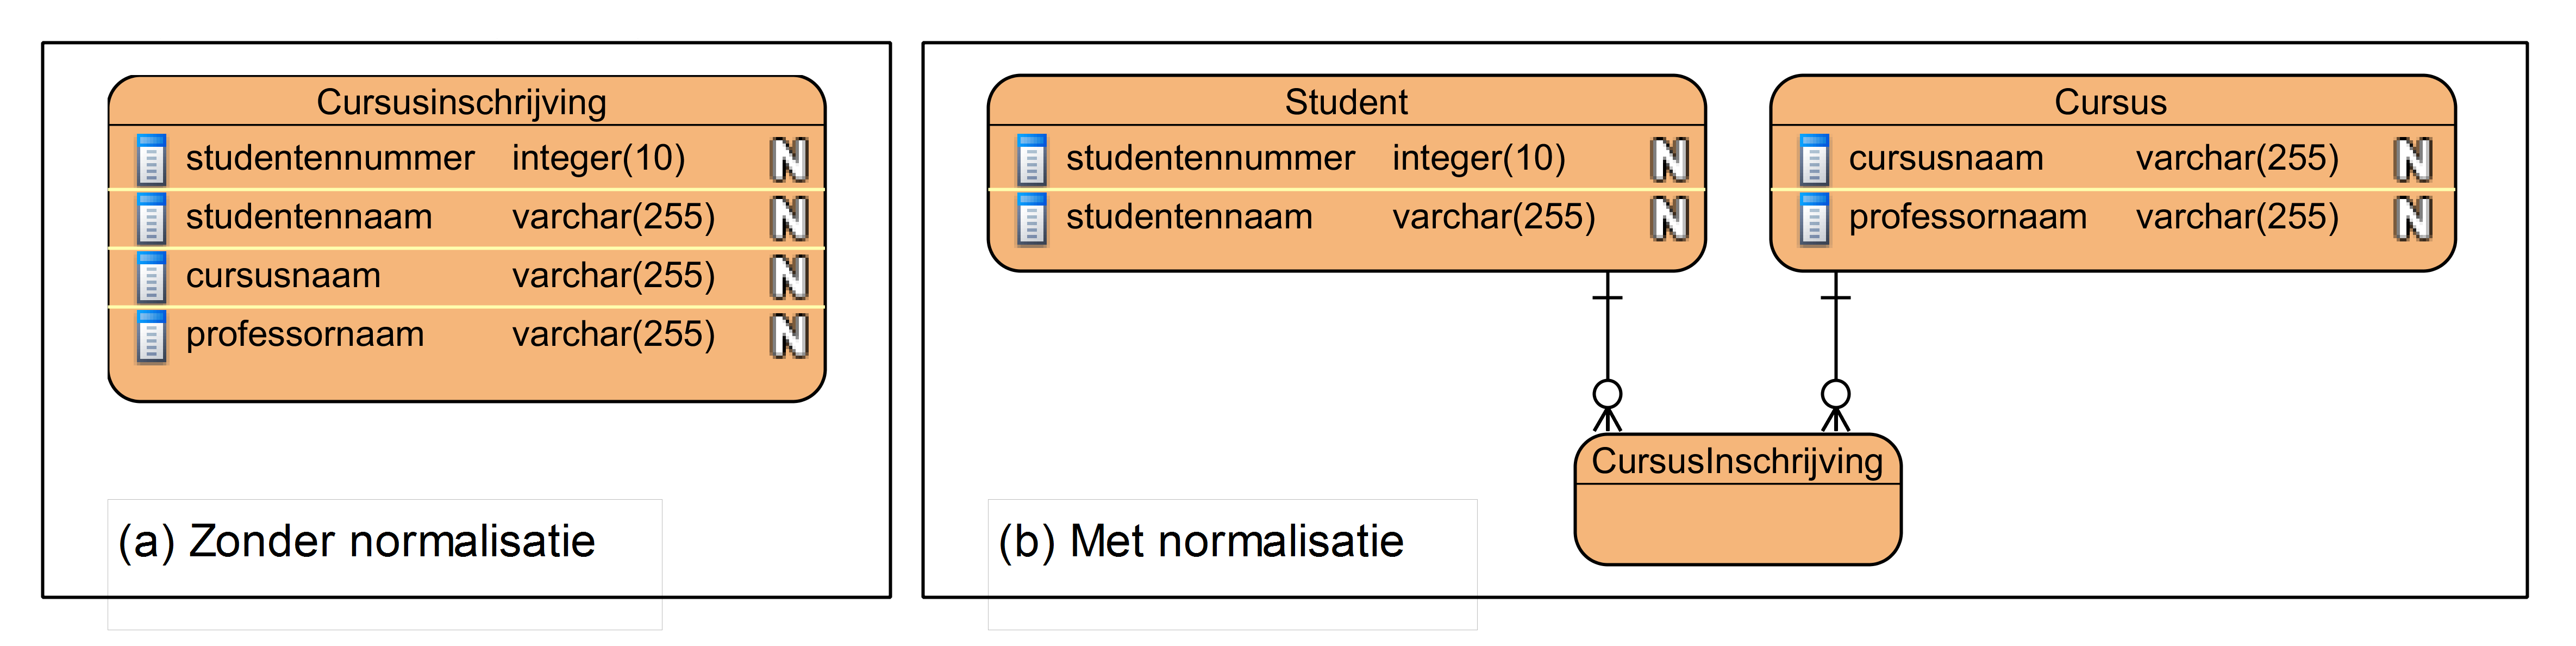
\includegraphics[width=\linewidth]{img/Relationeel-Model-Normalisatie.png}
\caption[Relationeel datamodel (a) zonder en (b) met normalisatie]{Relationeel datamodel (a) zonder en (b) met normalisatie}
\label{fig:Relationeel-Model-Normalisatie}
\end{figure}

Een belangrijk concept in een relationele database is ACID, welk voor betrouwbare en robuuste transacties zorgt

\paragraph{Atomair (\underline{A}tomicity)} Een database transactie moet oftewel volledig uitgevoerd worden oftewel heeft geen enkele bewerking plaatsgevonden. 

\paragraph{Consistent (\underline{C}onsistency)} Een transactie behoudt consistentie als de volledige uitvoering van de transactie de database van één consistente staat naar een andere brengt. Een consistente staat is een staat die ervoor zorgt dat waardes van een instantie consistent zijn met de andere waarden in dezelfde staat. Een voorbeeld is het overschrijven van \euro{50} van persoon A naar B, op het einde moet de totale som nog steeds gelijk zijn, A \euro{50} minder en B \euro{50} meer. Een inconsistente staat zou zijn dat enkel A \euro{50} minder heeft, maar B nog steeds evenveel. 

\paragraph{Geïsoleerd (\underline{I}solation)} Een transactie moet uitgevoerd worden alsof ze volledig voor of na andere transacties heeft plaatsgevonden. 

\paragraph{Duurzaam (\underline{D}urability)} Een voltooide transactie kan later niet ongedaan gemaakt worden.

Deze verschillende concepten bieden de garanties welke de gebruiker kan gebruiken voor zijn systeem. Daartegen over staat wel dat dit de complexiteit van de RDBMS groeit, ook indien dit voor bepaalde toepassingen misschien niet nodig is.

\subsection{NoSQL database\cite{Strauch.NoSQL}}\label{sec:eventualconsistency}
NoSQL DBMS zijn ontstaan door een groei en globalisering van de computersystemen en de bijhorende databases. Een RDBMS is gebouwd met een 'one size fits all'-gedachte, maar deze systemen hiermee complexiteit die voor bepaalde toepassingen niet nodig is. NoSQL systemen bestaan in verschillende variëteiten, elk met hun eigen eigenschappen en toepassingsgebied om zo de complexiteit te verminderen. Tussen deze verschillen is er een rode draad te vinden vergeleken met een RDBMS:
\begin{itemize}
	\item \textbf{Lagere complexiteit}: NoSQL systemen bieden minder opties en garanties dan de RDBMS, bepaalde applicaties hebben enkel nood aan een deel van de garanties. Bijvoorbeeld in een sociale netwerk moet een post niet onmiddellijk beschikbaar zijn voor al de vrienden van een persoon, maar dit mag even duren.
	\item \textbf{Hogere doorvoer}: Talrijke NoSQL systemen bieden een hogere doorvoer van data aan wat in veel gevallen een gevolg is van de lagere complexiteit of door de hulp van andere bewerkingen zoals MapReduce \cite{dean2008mapreduce}.
	
	\item \textbf{Horizontale schaalbaarheid en werkend op commodity hardware}: Waar grote RDBMS's werken met dure high-end systemen, was het bedoeling van NoSQL databases ondersteuning te bieden aan een veelvoud van geclusterde eenvoudige machines (commodity hardware). \\
	Horizontale schaalbaarheid staat voor het toevoegen extra machines aan een systeem voor extra resources, in tegenstelling tot verticale schaalbaarheid waar een krachtiger machine wordt gebruikt voor de opschaling. De horizontale opschaling wordt tot uitvoering gebracht door de data van een enkele database of tabel te verspreiden over verschillende machines die elk maar voor een deel van de data verantwoordelijk zijn en moeten opslaan.\\
	NoSQL systemen combineren deze twee elementen en bieden hierdoor een schaalbaar systeem aan met basis componenten.
	\item \textbf{Datamodel dichter bij objecten}: De meeste NoSQL systemen zijn zodanig ontworpen dat deze de vertaling van objecten naar opslag eenvoudiger maken t.o.v. RDBMS's. RDBMS zijn ontworpen voor het ontstaan van object georiënteerde programmeertalen en heeft de nood aan de vertaling van een object naar de databasestructuur. Bij het ontwerp van NoSQL werd er hiermee onmiddellijk rekening gehouden.  
\end{itemize}  \noindent
Deze verschillende argumenten leiden vervolgens tot BASE, een tegenreactie op ACID. \noindent 
\begin{itemize}
 \item Basis beschikbaarheid (\textbf{B}asically \textbf{Availability}): het DBMS biedt lees- en schrijfacties aan bij het falen van één of meerdere falende instanties. De ondersteuning is afhankelijk van systeem tot systeem samen met de configuratie
 \item \textbf{S}oft State: De data moet op een bepaald moment niet volledig consistent zijn. 
 \item Eventuele consistentie (\textbf{E}ventual Consistency): De database zal na enige tijd in een consistente status uitkomen, het is mogelijk dat oudere data tijdelijk leesbaar is. Eventuele consistentie kan op zijn beurt opnieuw onderverdeeld worden in 4 categorieën \cite[slide 16]{lipcon2009design}:
 	\begin{itemize}
 		\item \textit{Read your own writes} consistentie: Ongeachte van de server waarop een gebruiker leest, zal hij zijn schrijfactie onmiddellijk correct lezen. 
 		\item \textit{Session} consistentie: De gebruiker zal zijn schrijfactie onmiddellijk kunnen lezen binnen dezelfde sessie, een sessie is hierdoor meestal gelimiteerd tot een enkele database server. 
 		\item \textit{Casual} consistentie: Als een gebruiker versie X leest en vervolgens versie Y schrijft, zal elke gebruiker die versie Y leest ook versie X lezen.
 		\item \textit{Monotonic Read} consistentie: Dit levert monotone tijdsgaranties dat een gebruiker enkel recentere data versies in de toekomst zal lezen. 
 	\end{itemize}
\end{itemize}
De BASE eigenschappen kunnen gekoppeld worden aan de CAP theorie van Erik Brewer\cite{Brewer:2000:TRD:343477.343502}. CAP zegt dat een gedistribueerd systeem maar twee van de 3 CAP elementen kan ondersteunen: consistentie, beschikbaarheid en partitie tolerantie. De beschikbaarheid betekent dat bij het falen van een instantie er nog steeds schrijfbewerkingen mogelijk zijn. Bij partitie tolerantie kan het systeem overweg met het opgesplitst zijn van instantie door een niet werkende netwerk verbinding. De definitie van consistentie is hier anders als bij ACID: bij CAP is er sprake van consistentie als het DBMS zich gedraagt alsof er maar een enkel kopie van de data is.

\subsubsection{Classificatie van NoSQL systemen}
Er zijn vele NoSQL systemen ontworpen gedurende de laatste jaren, elk met hun eigen variëteit, functionaliteit en populariteit. Er bestaan verschillende manieren om de systemen te classificeren, maar één van de meest gebruikte doet dit op basis de data modellering. Een korte vergelijking op basis van deze bevindt zich in tabel \ref{table:selectie-classificatie}.  

\begin{table}[!h]
	\resizebox{\textwidth}{!} {
		\begin{tabular}{l l l l l l}
			\textbf{Soort} & \textbf{Performantie} & \textbf{Schaalbaarheid} & 			\textbf{Flexibiliteit} & \textbf{Complexiteit} & \textbf{Functionaliteit} \\ \hline
			Column & hoog & hoog & gematigd & laag & minimaal \\
			Document & hoog & variabel(hoog) & hoog & laag & variabel (laag) \\
			Graph & variabel & variabel & hoog & hoog & graph theory \\
			Key-Value & hoog & hoog & hoog & geen & variabel (geen) \\
		\end{tabular}
	}
	\caption{Classificatie en categorisatie van NoSQL DBMS's door Scofield en Popescu. \cite{categorizatie-sco10} \cite{categorizatie-pop10b} }
	\label{table:selectie-classificatie}
\end{table} 

\paragraph{Column Model}In een column-gebaseerd systeem wordt de data opgeslagen per kolom in plaats van de traditionele manier, per rij. Deze aanpak werd in eerste instantie gedaan voor analyse van business intelligentie. Het systeem is geïnspireerd door de paper van Google’s Bigtable \cite{chang2008bigtable}. \cite{Strauch.NoSQL}

\paragraph{Graph Model} In een grafen model, wordt de data voorgesteld en opslagen volgens de grafen theorie: knopen, lijnen en eigenschappen op de knopen en lijnen. \cite{bollacker2008freebase}.   

\paragraph{Key-Value Model} Key-Value systemen hebben een heel eenvoudig data model, data kan opgeslagen, opgevraagd en verwijderd worden op basis van een key. De informatie die in de database zit, is de waarde voor die key. \\
Met dit eenvoudig model en functionaliteit die weinig complexiteit introduceren, kan er gestreefd worden naar een hoge performantie, schaalbaarheid en flexibiliteit. \cite{Strauch.NoSQL}

\paragraph{Document Model} Document systemen zijn volgens vele de volgende stap in key-value systemen, waar deze complexere structuren toe laten, dit door middel van meerdere key/value paren per element. \cite{Strauch.NoSQL} \\
Een document moet geen vaste structuur hebben maar elk document op zich kan verschillende velden hebben, dit kan bijvoorbeeld toegepast worden bij boeken. Waar een bepaald boek een recept is, kan een ander een deel zijn van een trilogie. Bij het eerste kan de kooktijd opgeslagen worden en bij de tweede een referentie naar de andere boeken. \cite{Strauch.NoSQL}


\subsection{Bespreking van verschillende DBMS's}
Databases uit 4 categorieën komen verder aanbod, er is gekozen om de Graph NoSQL DBMS's niet te bespreken. Graph NoSQL DBMS's zijn bedoeld voor de opslag van data van grafen. Deze is significant verschillend van de andere categorieën en hierdoor niet opgenomen. 
 
\begin{itemize}
\item Column NoSQL DBMS's: Cassandra, HBase
\item Document NoSQL DBMS's: Apache CoucheDB, MongoDB
\item Key-Value NoSQL DBMS's: LightCloud (Tokyo), MemCache, Redis, Riak, Project Voldemort
\item Relationele DBMS's: MySQL, Pgpool-II (PostgreSQL)
\end{itemize}

Deze keuze van deze systemen is gebaseerd op de paper van Christophe Strauch \cite{Strauch.NoSQL}. Een korte bespreking van de verschillende systemen kan gevonden worden in bijlage \ref{sec:BesprekingDBMS}.


\section{Vergelijking van DBMS's naar performantie en CAP}
Bij de ontwikkeling van verschillende systemen is er een keuze naar welk DBMS er kozen wordt. De systemen verschillen en hebben elk hun eigen toepassingsgebied. Zoals besproken hierboven kan een opsplitsing naar het datamodel gemaakt worden, of in meer detail naar de ondersteunde database bewerkingen. 

Maar de systemen kunnen ook verschillende performantie of een keuze in het CAP theorema gekozen hebben.  In dit gedeelte zal er gekeken worden welke methodes er al beschikbaar zijn voor het kwantitatief vergelijken van de performantie, consistentie en beschikbaarheid en mogelijke resultaten. 

\subsection{Performantie benchmarking}
Indien men verschillende DBMS's wilt vergelijken bestaan er al enkele tools en studies om de performantie te kunnen vergelijken. Een blogpost van A. Popescu \cite{PopescuBenchmarkOverview} geeft een overzicht van verschillende benchmarking tools. 

Als eerste hebben vele DBMS's \textbf{interne benchmarking tools}, waarmee de database op verschillende configuraties kan getest en vergeleken worden. Deze resultaten zijn nuttig na de keuze van het DBMS. Het systeem kan getest worden bij het variëren van de parameters en het uitzoeken wat de bottleneck is in een bepaald systeem. Een voorbeeld hiervan is mongoperf\footnote{\url{http://docs.mongodb.org/manual/reference/program/mongoperf/}} voor MongoDB. 

Andere studies focussen op het testen van verschillende systemen en daarbij kunnen verschillende doelstellingen zijn: het ontwikkelen van een breed toepasbare tool, het testen van een grote verscheidenheid van DBMS's of het testen van een specifieke categorie van systemen. Elke van deze benchmarking brengt nieuwe kennis van de systemen maar heeft ook zijn beperkingen. Het totaal pakket van al de testen kan een gebruiker de informatie geven om een beter gefundeerde keuze te maken. 

Een eerste categorie van deze externe tools is het \textbf{ontwikkelen van een tool} voor verschillende systemen. Dit heeft als grote voordeel dat andere gebruikers nadien de testen opnieuw kunnen uitvoeren met de systemen in hun configuratie. Het is namelijk niet gegarandeerd dat het resultaat van een jaar geleden gelijkaard is met de nieuwste versie.
Het grootste nadeel is de testen die kunnen uitgevoerd worden, er is een grote variëteit aan systemen elk met hun eigen datastructuur en query mogelijkheden. De tool moet dus een gemeenschappelijke subset zoeken en enkel dit soort queries kunnen getest worden. Een voorbeeld van een dergelijke tool is YCSB\cite{cooper2010benchmarking}. Deze tool kan elk DBMS's testen zolang een basisset van 5 queries ondersteund wordt: het invoegen, updaten, verwijderen en opvragen van een enkel record met daarnaast ook de mogelijkheid tot scan queries, met behulp van 1 query een verzameling van records tegelijk op te vragen. \\
Sommige systemen ondersteunen bepaalde queries niet rechtstreeks maar bevatten wel de functionaliteit om deze met behulp van meerdere achtereenvolgende bewerkingen te implementeren. Bijvoorbeeld een update kan geïmplementeerd worden door het opvragen, verwijderen en vervolgen invoegen van het aangepaste record. 

Een volgende categorie zijn de \textbf{resultaten van gerelateerde DBMS's}, dit zijn voornamelijk systemen met hetzelfde datamodel. Het grote voordeel hieraan is dat deze systemen in de meeste gevallen een vrij gelijkaardige set aan query mogelijkheden bevatten waardoor er meer diepgang is dan tussen meer verschillende systemen. Een voorbeeld van zulk onderzoek is gedaan door P. Pirzadeh et al\cite{pirzadeh2011performance} voor de key-value systemen, meer specifiek is er gefocust op het uitvoeren van range queries tussen Cassandra, HBase en Voldemort.  \\
In deze categorie vallen ook de resultaten die meestal getoond worden op de website van de DBMS's, een vergelijkende benchmark met andere soortgelijke systemen. Hoewel de resultaten niet altijd volledig objectief zijn, kan de gevolgde test methode wel interessant zijn. Een voorbeeld van deze studie is de Key-Value benchmarking van VoltDB\cite{huggkey} waar Cassandra en VoltDB vergeleken worden, een belangrijke kanttekening is dat de auteur zelf al aanhaalt dat de systemen vrij verschillend zijn.

Als laatste categorie, zijn er de \textbf{resultaten van verschillende DBMS's} waar verschillende soorten systemen met elkaar getest worden. De belangrijkste voordeel is dat er resultaten zijn die verschillende soorten met elkaar vergelijken en waardoor niet alleen verschillen in het datamodel kunnen vergeleken worden in toekomstige studies maar ook performantie verschillen. Het nadeel is dat er een gemeenschappelijke subset gevonden moet worden, hierdoor kunnen bepaalde databases hun kracht net niet laten zien. Enkele van deze onderzoeken zijn \cite{tudorica2011comparison} en \cite{rabl2012solving}. Deze laatste maakt gebruik van de YCSB tool die hierboven besproken was. 


\subsection{Consistentietesten}
Bij een gedistribueerd systeem kunnen er verschillende keuzes gemaakt worden naar synchrone of asynchrone replicatie en welk soort consistentie er aangeboden wordt. In de documentatie van DBMS's worden er beloftes gemaakt, maar hoe is de consistentie in de realiteit?

Een recent artikel \cite{golab2014eventually} (maart 2014), stelt dat er momenteel nauwelijks gekwantificeerde methodes bestaan om de eventuele consistente te meten. In hun artikel stellen zij twee mogelijke methoden voor: de actieve of passieve analyse. \\
De \textbf{actieve} analyse bestaat uit het wegschrijven van data waarna men hoe lang het duurt vooraleer alle servers de nieuwe waarde hebben. 
Bij de \textbf{passieve} analyse kijkt men langs de gebruikerskant. Leest de gebruiker altijd de laatste waarde (=strikte consistentie)? Is het mogelijk dat een nieuwe waarde al wordt gelezen voor de schrijfactie voltooid is? \\
Beide analyses hebben hun eigenschappen, de actieve analyse is gericht op het database systeem en zijn server. 
Bij de passieve analyse is georiënteerd naar de gebruiker toe, hoe moet deze zijn toepassingen aanpassen, wat zijn de garanties die geleverd worden aan de gebruiker? 

Voornamelijk naar actieve analyse is er al kwantitatief onderzoek verricht. Onder andere Duitse onderzoekers hebben op het Amazon S3 platform getest hoe lang het duurt vooraleer data geschreven in MiniStorage beschikbaar is voor alle gebruikers op al de verschillende servers. \cite{bermbach2011eventual}. \\
Daarnaast zijn er ook 2 interessante resultaten gevonden: allereerst heeft het Amazon S3 systeem geen monotone lees consistentie, daarnaast bleek het inconsistentie interval voor een bepaald record periodiek verloop te hebben dat niet door de onderzoekers verklaard konden worden. 

De YCSB software van hierboven is door onderzoekers in de VS uitgebreid naar YCSB++\cite{patil2011ycsb++} waardoor deze meer ondersteuning heeft voor het meten van systeembelasting maar ook voor de consistentie-eigenschappen. Enkele geteste systemen zijn in principe strikt consistent, zoals HBase, maar deze worden eventueel consistent door het gebruiken van buffers bij de gebruiker. Vervolgens testen zij hoe lang het duurt voor de data ook gelezen kan worden. De vertraging is sterk afhankelijk is van het aantal acties van de schrijvende gebruiker: indien er meer geschreven wordt, zal de buffer sneller verzonden worden naar de server en dus sneller beschikbaar zijn voor andere gebruikers. \\
Hoewel zij stellen dat er ook testen zijn gedaan naar eventuele consistentie voor Cassandra en MongoDB, zijn de resultaten niet beschikbaar in het artikel of op de website. 

Andere onderzoeker\cite{wada2011data} doen analyse op Amazon SimpleDB. In de situatie wordt getest of de database read-your-own-writes en monotone consistentie ondersteund. Aan het eerste is niet voldaan met \textit{eventual consistency read}. Met minder dan 500 ms tussen het einde van de schrijfactie en het begin van de leesactie, wordt er slechts 33\% van de nieuwe data gelezen, zodra er meer als 500 ms gewacht wordt, gaat dit naar 99\%. Ook is er geen monotone consistentie omdat er van verschillende servers kan gelezen worden bij opvolgende leesacties, sommige zullen de data al wel hebben, anderen niet. 

Bij Netflix heeft men aan passieve analyse gedaan op hun Cassandra systeem \cite{kalantzisnetflix} waar zij in hun testen geen consistentieproblemen vonden naar de gebruiker toe. Er is geen vermelding hoeveel vertraging er zit tussen beide transacties. Volgens hun gaat het meer om de perceptie dat data verkeerd kan gelezen worden en de angst van het middle management. 

\subsection{Beschikbaarheidstesten}
Een derde verschilpunt is hoe de systemen omgaan met het falen van een enkele server en dit onder verschillende opties: Het is mogelijk dat deze tijdelijk uitgeschakeld wordt wegens onderhoud. Het kan gaan om een onverwachte crash van de software op een server of een crash van een volledige server, tenslotte kunnen er ook nog netwerkproblemen optreden waardoor deze (tijdelijk) niet beschikbaar is. 

Nu hoe gaan deze systemen om het falen en terug online brengen van de systemen? Zijn er geen acties mogelijk op de server, worden de connecties tijdelijk verbroken, is er een verhoogde of verlaagde vertraging op de transacties? Detecteert het systeem automatisch wanneer de oorspronkelijke server terug online komt of moet gemeld worden om de server terug te gebruiken? In een NoSQL DBMS waar gewerkt wordt commodity hardware, zal het falen regelmatig gebeuren en verschillende systemen reageren anders op deze acties. 

Uit de literatuurstudie zijn er geen vergelijkende studies voor database systemen gevonden. Er is voor de meeste DBMS's informatie te vinden op de website hoe zij in een gedistribueerde omgeving werken zoals het al dan niet gebruik van sessies en de duur van een sessie. Maar voor het effect in de praktijk, is het handmatig testen. 

\section{Doelstelling en bijdrage}\todo{Loop hier nog is over}
In de literatuurstudie komt naar voor dat er een gebrek is aan kwantitatieve methodes om DBMS's te vergelijken naar consistentie en beschikbaarheid. 

Het eerste doel van deze thesis is om benchmark te ontwikkelen die het gedrag in de praktijk kan testen. Deze testen zullen het uitvallen van een service, server en netwerk simuleren voor de beschikbaarheidstesten. Bij de consistentietesten wordt er een tool aangeleverd die verschillende types van eventuele consistentie kan testen. 

Daarnaast zal aangetoond worden dat de testmethode werkt door het toepassen op drie voorbeeldsystemen: HBase, MongoDB en Pgpool-II(uitbreiding van PostgreSQL). Door het kiezen van verschillende systemen met een verschillend datamodel, kan de testmethode een kwantitatieve vergelijking ten opzichte van elkaar mogelijk maken. 

Tenslotte is het doel om de testen eenvoudig te kunnen uitvoeren voor andere gebruikers, op deze manier kan de data gecontroleerd worden. Daarnaast wordt er ook de mogelijkheid aangeboden om nieuwere versies en andere infrastructuren te kunnen testen.

Met deze drie doelstellingen wordt er een testmethode, een werkende benchmarking tool en resultaten aan een gebied waar er nog nauwelijks kwantitatieve methodes zijn. 

\section{Conclusie}
Deze thesis zal handelen over het ontwikkelen en uitvoeren van een benchmark systeem voor consistentie en beschikbaarheid naar relationele en NoSQL databases. Momenteel zijn er weinig kwantitatieve methodes en resultaten naar beschikbaarheid en consistentie.  

In het vervolg van deze tekst, zal in hoofdstuk \ref{sec:methodiekvantesten} een algemene testmethode voor consistentie en beschikbaarheid voorgesteld worden. In hoofdstuk \ref{sec:implementatie} wordt besproken hoe de voorgestelde methode in de praktijk geïmplementeerd wordt. Daarna worden de observaties voorgesteld in hoofdstuk \ref{sec:observaties} met een analyse en verklaring van de observaties in hoofdstuk \ref{sec:analyse}. Een conclusie volgt tenslotte in hoofdstuk \ref{sec:conclusie}. 
\chapter{Methodiek van de testen}




\chapter{Implementatie}

\section{Selectie van de DBMS}

\subsection{Selectiecriteria voor DBMS}
Bij de selectie van de systemen of een systeem een bepaalde eigenschap al dan niet ondersteunt. In het totaal zijn er 5 verschillende eigenschappen waarop wordt geselecteerd. 

\paragraph{Vrije software} Om testen tussen verschillende DBMS te kunnen vergelijken op een gelijkaardige infrastructuur, is het nodig dat deze software kan geïnstalleerd worden op de eigen infrastructuur. Daarnaast is er in dit onderzoek gekozen voor gratis beschikbare software. 

\paragraph{Persistentie} Voor het testen van de beschikbaarheid van de data, is het een voordeel dat de data op harde schijf aanwezig is: bij herstel dient er minder data over het netwerk gestuurd te worden. Om deze reden hebben deze systemen een voorkeur op systemen die de data enkel in geheugen houden. 

\paragraph{Replicatie} Eén van de testen is de beschikbaarheidstest, indien de data maar op een enkele server opgeslagen is, zal de data op de uitgeschakelde server niet langer beschikbaar zijn. Met replicatie zal de data op verschillende servers opgeslagen worden en zal de data nog steeds beschikbaar zijn in het geval van een enkele uitgeschakelde server. 

\paragraph{Data distributie} Het is de bedoeling om systemen te testen die een grote hoeveelheid data kunnen opslaan. Om aan deze vereiste te voldoen, is het nodig dat elke server niet al de data opslaat bij een voldoende hoog aantal servers (bij weinig servers, is elke server nodig om aan de replicatie vereiste te voldoen)

\paragraph{Ondersteuning voor verschillende query methodes} Bij de testen worden er 5 soorten queries uitgevoerd: invoegen, aanpassen, verwijderen en opvragen van een individueel record en het opvragen van meerdere queries. De DBMS moet ondersteuning voor deze queries. De eerste 4 kunnen in al de systemen geïmplementeerd worden met één of meerdere queries. Maar het opvragen van meerdere queries is in bepaalde systemen niet mogelijk en deze worden om deze reden niet behandeld. 


\begin{table}
    \begin{tabular}{lll|l|l|l|l|l|l|l|l|l}
    ~                & ~         & \multicolumn{2}{l}{ \rotatebox[origin=c]{90}{Column database}} & \multicolumn{2}{l}{\rotatebox[origin=c]{90}{Document database}} & \multicolumn{4}{l}{\rotatebox[origin=c]{90}{Key-Value database}} & \multicolumn{2}{l}{\rotatebox[origin=c]{90}{Relationele database}} \\
    ~                & ~         & \rotatebox[origin=c]{90}{Cassandra} & \rotatebox[origin=c]{90}{HBase} & \rotatebox[origin=c]{90}{Apache CouchDB} & \rotatebox[origin=c]{90}{MongoDB} & \rotatebox[origin=c]{90}{Lightcloud (Tokyo)} & \rotatebox[origin=c]{90}{Memcache} & \rotatebox[origin=c]{90}{Riak} & \rotatebox[origin=c]{90}{Voldemort} & \rotatebox[origin=c]{90}{MySQL} & \rotatebox[origin=c]{90}{Pgpool-II (PostgreSQL)} \\
    \multicolumn{2}{l}{Persistentie} & ~               & ~     & ~                 & ~       & ~                  & ~        & ~    & ~         & ~                    & ~                      \\
    \multicolumn{2}{l}{Replicatie} & ~               & ~     & ~                 & ~       & ~                  & ~        & ~    & ~         & ~                    & ~                      \\
    \multicolumn{2}{l}{Data distributie} & ~               & ~     & ~                 & ~       & ~                  & ~        & ~    & ~         & ~                    & ~                      \\
    Query soort      & Aanpassen & ~               & ~     & ~                 & ~       & ~                  & ~        & ~    & ~         & ~                    & ~                      \\
    ~                & Range     & ~               & ~     & ~                 & ~       & ~                  & ~        & ~    & ~         & ~                    & ~                      \\
    \end{tabular}
    \caption{Ondersteuning van de besproken DBMS naar de selectie criteria}
\end{table}
\subsection{Vergelijking van de DBMS}
% A table for each category

\subsection{Architectuur geselecteerde DBMS}
\subsubsection{HBase}
\subsubsection{MongoDB}
\subsubsection{Pgpool-II (PostgreSQL)}

\section{Selectie en uitwerking van de testsoftware}


\section{Installatie van de DBMS en testsoftware}

%Uitleggen van gebruik van YCSB
\subsection{Automatische installatie met IMP}

\subsubsection{YCSB!}
\subsubsection{HBase}
\subsubsection{MongoDB}
\subsubsection{Pgpool-II (PostgreSQL)}

\section{Uitvoeren van de calibratie en testen}

\section{Verzamelen en analyse van de testresultaten}
\chapter{Observaties}
In dit hoofdstuk worden de resultaten getoond van de testen die zijn uitgevoerd, met een bespreking van de speciale elementen. Er zullen nog geen redenen aangehaald of conclusies getrokken worden, dit wordt in het volgende hoofdstuk gedaan. 

De resultaten zullen besproken worden per testsoort: eerst de resultaten voor de calibratie daarna voor beschikbaarheid en tenslotte voor consistentie. De figuren bevinden zich in bijlage \ref{sec:figobservaties}

De ruwe testdata kan geraadpleegd worden op \url{https://github.com/thuys/YCSB-Testdata}. 

\section{Calibratie}

\paragraph{Aantal gebruikers}
De resultaten van de calibratietest voor het aantal gebruikers kunnen gevonden worden in figuur \ref{fig:calibratie-gebruikers-resultaat}. Op de x-as is het gemiddeld aantal queries per second getoond over een periode van 600s, op de y-as de gemiddelde vertraging. De verschillende punten stellen een aantal gebruikers voor die zijn aangegeven met het bijhorend getal. 

Het aantal gebruikers wordt zo gekozen dat het totale aantal queries zakt of voor een sterke groei in vertraging zorgt, dit zorgt voor de gegevens in tabel \ref{table:calibratie-gebruikers-resultaat}. Bij MongoDB is er voor een lage waarde van 15 gebruikers gekozen, in plaats van 50, de reden hiervoor is dat de variatie in de vertraging groter wordt bij meer gebruikers, wat de data van de overige testen potentieel minder stabiel maakt.  

\begin{table}[h!]
	\centering
	\begin{tabular}{l| l }
		\textbf{DBMS} & Aantal gebruikers \\
		\hline
		HBase & 50 \\
		MongoDB & 15\\
		Pgpool-II & 30\\
	\end{tabular}
	\caption{Calibratie: Aantal gebruikers per test voor de verschillende DBMS's}
	\label{table:calibratie-gebruikers-resultaat}
\end{table}

\paragraph{Aantal queries per seconde}
De resultaten voor de calibratietest voor het aantal queries per seconden kunnen gevonden worden in de figuren \ref{fig:calibratie-queriesperseconde-hbase}, \ref{fig:calibratie-queriesperseconde-mongodb} en \ref{fig:calibratie-queriesperseconde-pgpool-ii} voor respectievelijk HBase, MongoDB en Pgpool-II. Deze figuren tonen in de bovenste figuur de gemiddelde vertraging op een query afhankelijk van het aantal queries per seconde, naarmate het aantal queries toeneemt stijgt de vertraging, met uitzondering van een laag aantal queries. De onderste figuur toont op de y-as de verhouding tussen het eigenlijk aantal uitgevoerde queries per seconde t.o.v. het gevraagde aantal queries per seconde. Een fictief voorbeeld: bij het vragen van 100 queries/sec wordt er in de praktijk maar 60 uitgevoerd, dit zorgt voor een waarde van $0.6$. 

Met beide figuren samen, kan een matige belasting gekozen. Een matige belasting is een belasting waarbij de onderste figuur de waarde 1 zo dicht mogelijk benaderd en de vertraging nog niet te veel is gestegen t.o.v. van een lage belasting. De gekozen waarde zijn te vinden in tabel \ref{table:calibratie-queriesperseconde-resultaat}. 

\begin{table}[htb!]
	\centering
	\begin{tabular}{l| l }
		\textbf{DBMS} & Aantal requests per seconde \\
		\hline
		HBase & 600 \\
		MongoDB & 200\\
		Pgpool-II & 100\\
	\end{tabular}
	\caption{Calibratie: Aantal queries per seconde per test bij een matige belasting voor de verschillende DBMS's.}
	\label{table:calibratie-queriesperseconde-resultaat}
\end{table}



\section{Beschikbaarheidstest}
Bij de beschikbaarheidstesten kunnen de gegevens op verschillende manieren voorgesteld worden: de vertraging per query over de hele test, de vertraging tijdens het stoppen en starten van systemen of een vergelijking van de vertraging voor het stoppen (150-250s), na het herstarten (700-800s) en tussen het stoppen en starten(400-500s). 

Voor elk van de systemen is voor al de acties op de verschillende instanties data in voorhand, maar slechts enkele grafieken zullen getoond worden. Al de grafieken kunnen gevonden worden op GitHub op de link gegeven in het begin van het hoofdstuk. 

Een punt op de grafiek stelt de gemiddelde vertraging van 1 seconde voor, de lijn het gemiddelde over 10 seconden. 

\paragraph{HBase}
Bij HBase zijn er verschillende reacties op het stopzetten van een node. Bij het zacht stoppen van een instantie, is er een onderbreking van gemiddeld ongeveer 20 seconde in de testen. Daarna kunnen er nog verhogingen in de queries af en toe optreden. Zie figuur \ref{fig:beschikbaar-hbase-soft}. 

Bij de netwerk onderbreking is er in de testen een onderbreking van gemiddeld ongeveer 100 seconden. Daarna is het terug stabiel. Zie figuur \ref{fig:beschikbaar-hbase-drop}

Bij een harde stop is er een combinatie van de netwerk onderbreking én is het af en toe zo dat de volledige periode geen queries mogelijk zijn. Zie figuur \ref{fig:beschikbaar-hbase-drop} en \ref{fig:beschikbaar-hbase-hard}

Tijdens de onderbreking (400-500s), is er geen significante verandering in de vertraging van de uitgevoerde queries gemeten (t.o.v. 150-250s en 700s - 800s). 


\paragraph{MongoDB}
Ook bij MongoDB zijn er verschillende reacties op het stopzetten als men de queries onder standaard configuratie uitvoert. In het geval van zacht of hard stoppen is er geen verschil in de reactie, bij 2/3 van de keren is er geen verschil merkbaar, bij 1/3 van de keren is er tijdelijke verhoging van de vertraging, een voorbeeld toont dat de scan operatie voor 2 seconden uitgesteld wordt. Figuur van het overzicht: \ref{fig:beschikbaar-mongodb-soft} met een zoom naar de stop \ref{fig:beschikbaar-mongodb-soft-zoom}.

Bij het onderbreken van het netwerk is er in bepaalde geen significante verandering, op andere momenten is een gedrag soortgelijk aan dat bij een zachte stop te merken. In andere gevallen is het zo dat er geen queries mogelijk zijn gedurende de volledige netwerk onderbreking. Zie figuur \ref{fig:beschikbaar-mongodb-drop}. 

Tijdens de onderbreking (400s- 500s), is er geen significante verandering in de vertraging van de uitgevoerde queries gemeten (t.o.v. 150-250s en 700s - 800s). 
 


\paragraph{Pgpool-II} Bij Pgpool-II is een green verschil tussen een harde of zacht stop. In beide gevallen is er tijdelijk een onderbreking van al de queries, er is een verhoogde vertraging van ongeveer 2 seconden, een voorbeeld bevindt zich in figuur \ref{fig:beschikbaar-pgpool-soft}. 

Bij een netwerk onderbreking, zijn er enige tijd geen queries mogelijk en na 30 seconden was de onderbreking over in de testen. Een voorbeeld bevindt zich in figuur \ref{fig:beschikbaar-pgpool-netwerk}.  

Tijdens de onderbreking is er een verandering naar schrijfbewerkingen toe, deze nemen significant minder tijd in beslag, dit geldt niet voor leesbewerkingen. Voorbeelden uit de testen bevinden zich voor beiden in figuren \ref{fig:beschikbaar-pgpool-boxplot-read} en \ref{fig:beschikbaar-pgpool-boxplot-write}. 

De herstel van een server na deze opnieuw online gebracht hebben, lukt slechts in zeldzame keren na deze te hebben opstarten. Enkel als alle connecties zijn, verbroken lukt het herstel. 

\section{Consistentie test}
Voor de consistentie testen worden er empirische verdelingsfuncties gebruikt. Dit zijn functies waarbij op de y-as het percentage van de waarden kleiner dan x staat aangegeven.

Voor de consistentie testen wordt er op de x-as de start- en/of stoptijdstippen van de verschillende soorten getoond. Het verschil tussen de y-waarde van de start- en stoptijdstippen geeft aan hoeveel queries er op dat moment uitgevoerd worden. De startmomenten van een lezer zijn de eerste keer dat deze de correcte data leest. 

\paragraph{HBase}
Bij HBase is er geen verschil tussen het invoegen of aanpassen van data naar consistentie, dit zijn dezelfde queries. Daarnaast zijn er geen configuratie mogelijkheden voor het lezen of schrijven van data naast het in- of uitschakelen van de caches aan de gebruikerskant, deze uitgeschakeld zijn al de testen. 

Figuur \ref{fig:consistentie-hbase-start} toont een overzicht van de verschillende starttijdstippen voor het lezen van consistente data. Figuur \ref{fig:consistentie-hbase-R1} toont de start- en eindtijdstippen voor lezer 2 naast deze voor de schrijver. De maximale waarde van de x-as is zo gekozen dat voor elke dataset minstens 99\% van de data getoond is. 



\paragraph{MongoDB} Bij MongoDB zijn er 5 soorten lees- en 5 soorten schrijfconfiguraties mogelijk. Na de testen bleek het dat secondarypreferred gelijk was aan secondary en is niet getoond in de grafieken om deze reden. 

Voor elk van de 5 mogelijke schrijvacties, is een overzicht gegeven in figuren \ref{fig:consistentie-mongodb-all} en \ref{fig:consistentie-mongodb-R2}. In de eerste figuur, is de data van al de lezers gecombineerd, bij de tweede wordt er enkel naar lezer 2 gekeken. De maximale waarde van de x-as is zo gekozen dat voor elke dataset minstens 97\% en 99\% van de leesdata is getoond inor respectievelijk figuur \ref{fig:consistentie-mongodb-all} en \ref{fig:consistentie-mongodb-R2}. Er zijn telkens de update queries getoond met een vergelijking tussen de insert en update bij majority. Ook uit de andere data blijkt dat deze niet significant verschillend zijn. 

Een vergelijking van de duur van de verschillende leesoperaties kan gevonden worden in figuur \ref{fig:consistentie-mongodb-all-mongodb-write} waar er minstens 90\% van de leesdata is getoond. 


\section{Conclusie}
De resultaten zijn verschillend voor de verschillende systeem, in het volgend hoofdstuk zullen de resultaten geanalyseerd worden en mogelijke verklaringen gezocht worden. 

\chapter{Analyse van de resultaten}\label{sec:analyse}
In dit hoofdstuk worden de observaties in meer detail besproken. Voor elke observatie zal er geprobeerd worden een verklaren te vinden of een hypothese voor te stellen. 

Eerst zal de kalibratie aan bod komen, vervolgens de beschikbaarheids- en tenslotte de consistentietesten. Bij elke test zullen eerst de verschillende systemen besproken worden om vervolgens een vergelijking te maken. 

\section{Kalibratie}
Over de kalibratie testen valt in het algemeen niet veel af te leiden, de verschillende systemen hebben niet hetzelfde aantal instanties, zo heeft Pgpool-II slechts 3 instanties t.o.v. 6 voor MongoDB. 

Enkel op de stijgende variatie van de vertragingen in MongoDB zal dieper ingegaan worden. Bij het toenemen van het aantal gelijktijdige gebruikers neemt niet enkel de gemiddelde vertraging toe, maar ook de standaard deviatie groeit significant. Sommige bewerkingen verlopen snel, andere bewerkingen staan zeer lang in de wachtrij. De reden hiervoor is een lezers/schrijvers locking systeem op de gehele database\cite{mongodb-concurrency}. Hierdoor zorgt een leesactie voor de blokkering van alle schrijfactie op de database en vice versa. Naar mate er meer gebruikers zijn, kunnen er meer opeenvolgende schrijfoperaties zijn, dit zal de leesacties langer blokkeren. Maar indien alle gebruikers samen lezen, kan dit parallel gebeuren, een grotere variatie in de vertraging treedt hierdoor op. \\
Het gevolg van deze werkwijze is dat indien veel gebruikers actief zijn, de duur van een bewerking moeilijk te voorspellen is. Voor de resultaten van de benchmarking tool is het best om zo weinig mogelijk variatie binnen een testrun te hebben, vandaar is er gekozen voor weinig gelijktijdige gebruikers.

\section{Beschikbaarheidstest}
Bij de beschikbaarheidstesten blijkt er uit de resultaten dat de verschillende systemen een andere aanpak hebben genomen. Voor elk systeem zullen de drie testen in detail besproken worden, daarna zal een vergelijking tussen de drie systemen besproken worden. 

\paragraph{HBase} Bij HBase heeft een bepaalde HRegionServer de verantwoordelijkheid over een Regio voor een bepaalde tijd. Dit is een sessie dit door HMaster uitgedeeld wordt en bijgehouden wordt in Zookeeper. Deze sessie kan vroegtijdig beëindigd worden door de HRegionServer of er moet gewacht worden tot deze verlopen is, enkel op die momenten kan er een nieuwe HRegionServer aangeduid worden. Dit zorgt voor een duidelijk verschil tussen een zachte stop, een harde stop of een netwerk onderbreking. 

De duur van een sessie kan geconfigureerd worden in Zookeeper en staat standaard op 180 seconden. \cite{hbase-doc}. 

\subparagraph{Zachte stop} Indien een RegionServer wordt stopgezet, nemen de queries tijdelijk meer tijd in beslag. Na het stopzetten van de RegionServer is er in bepaalde gevallen een verhoogde vertraging in beide leesoperaties (scan en lees). \\ 
Het stopzetten van een HRegionServer is enkel merkbaar als er data gelezen of geschreven wordt waarvoor deze server verantwoordelijk is. In de testen worden vele bewerkingen per seconde uitgevoerd per connectie. De kans dat de HRegionServer gecontacteerd wordt kort na het stopzetten is daarom zeer groot. \\
Zodra er een herverdeling is van de HRegions over de aanwezige HRegionservers, verdwijnt deze verhoogde vertraging. De onderbreking neemt enkele seconden in beslag. 

\subparagraph{Netwerk onderbreking} Bij een netwerk onderbreking, worden de queries tijdelijk stopgezet en falen de queries in tussentijd. Deze onderbreking duurt significant langer, tot 180 seconden, dan in het geval van een zachte stop. Dit komt doordat de regio's pas kunnen toegewezen worden na het verlopen van hun sessie.  

\subparagraph{Harde stop} Bij het stopzetten van een instantie op de harde manier, zijn er twee reacties: de eerste is vergelijkbaar met deze van een netwerk onderbreking. De andere laat pas opnieuw queries toe na het herstellen van het netwerk verkeer. In een manuele test bleek dit opgelost te zijn na het verbreken van de connectie en het opnieuw verbinden, maar de oorzaak waarom deze permanente onderbreking af en toe ontstaat, is niet gevonden. 

\subparagraph{Herstel van de instantie} Het herstel van de server zal automatisch op een asynchrone manier gebeuren. Er valt te configureren hoeveel netwerkverkeer er maximaal per seconde zal worden gebruikt voor de synchronisatie. Het herstel is niet merkbaar voor de gebruiker op de vertraging van de bewerkingen. 

\paragraph{MongoDB} Bij MongoDB is er tussen de leden van een Replicaset een heartbeat protocol. Indien er gedurende 10 seconden geen antwoord op een een heartbeat komt, wordt een server als offline bestempeld. De server die als laatste contact met de primary heeft gehad zal zijn rol overnemen indien de primary onbereikbaar wordt\cite{mongodb-manual}. Dit heeft zijn invloed op de verschillende manieren om een server stop te stopzetten. 

\subparagraph{Zachte stop en harde stop} Bij een zachte of harde stop is er een kans van 1 op 3 dat het uitvallen van een instantie zichtbaar is, dit is te verklaren doordat een replicaset bestaat uit drie server in onze configuratie. In de standaard modus wordt er enkel gelezen naar en geschreven van de primary, indien deze onbereikbaar wordt is er een onderbreking. Na het kiezen van een nieuwer primary is er geen verschil in vertraging per soort query ten opzichte van ervoor. Er zijn 2 hypothesen waarom een harde stop op dezelfde manier reageert: bij een harde stop wordt de sessie nog altijd vrijgegeven, of er zijn verkiezingen voor een nieuwe primary voordat de sessie van de oude primary is afgelopen. Deze hypothesen zijn niet getest of verder onderzocht. 

\subparagraph{Netwerk onderbreking} Bij een netwerk onderbreking zou het te verwachten zijn dat na maximaal 10 seconde de primary zou veranderen. Onder de aangelegde belasting blijkt dat de database heel de tijd onbeschikbaar tot de primary opnieuw bereikbaar is via het netwerk. Bij het manueel testen blijkt dat er dezelfde foutmelding gegeven wordt als bij het stoppen van de database, maar dat de data onbeschikbaar is. Het volstaat om de verbindingen af te sluiten en opnieuw aan te maken om het probleem op te lossen. Er is geen reden gevonden voor dit gedrag. 

\subparagraph{Herstel van de instantie} Het herstel van de server zal automatisch op een asynchrone manier gebeuren. Dit is niet merkbaar voor de gebruikers en de server zal als secondary ingezet worden. 

\paragraph{Pgpool-II} Bij Pgpool-II wordt de status van de PostgreSQL instanties getest wanneer er een gebruiker actief is.  Bij het uitvallen van een instantie en opnieuw opstarten terwijl er geen gebruiker verbonden is met Pgpool-II, zal dit niet opgemerkt worden. Daarnaast zijn er verschillende reacties op de geteste scenario's. 

Een vereiste bij het herstellen van een instantie is dat er op dat moment geen enkele verbinding met de router instantie is. 

\subparagraph{Zachte stop} Bij een zachte stop van een data instantie worden alle verbinden van de gebruikers met Pgpool-II onmiddellijk verbroken. Nadien kan er terug verbonden worden met Pgpool-II. In deze omgeving gaan nadien de verschillende schrijfoperaties sneller omdat deze niet meer gerepliceerd moeten worden. Een hypothese is dat bij een grote hoeveelheid data instanties dit effect kleiner zal worden.  

\subparagraph{Harde stop} Een harde stop reageert hetzelfde als een zachte stop. Dit omdat ook hier de connecties onmiddellijk verbroken zijn. Het besturingssysteem van de data instantie zal antwoorden dat er geen service op de poort aan het luisteren is en Pgpool-II detecteert de fout. 

\subparagraph{Netwerk onderbreking} Bij een netwerk onderbreking is er een ander gedrag, de queries wachten op een antwoord maar krijgen dit niet. Hierdoor worden alle bewerkingen geblokkeerd tot een antwoord of de time-out van de connecties naar de dataserver die standaard 30 seconde is. In dit geval is er een time-out en gebeurt de interne overschakeling. Hierbij worden alle connecties van de gebruikers verbroken en de onbereikbare server niet meer gebruikt. Daarna kan de gebruiker opnieuw verbinden met Pgpool-II en queries uitvoeren. 

\subparagraph{Vermindering van schrijfvertraging} De reden tot de vermindering van de schrijfvertraging is te verklaren door de wijze waarop Pgpool-II de schrijfbewerkingen uitvoert. Deze zullen eerst op de master uitgevoerd worden en vervolgens op de verschillende slaves. Bij het wegvallen van een instantie is er in de testopstelling nog maar een enkele dataserver over, hierdoor duurt een schrijfactie maar half zo lang. De leesacties duren ongeveer even lang aangezien er nog steeds gelezen wordt van een dataserver. 

\subparagraph{Herstel van de instantie} Bij het opnieuw inschakelen van een instantie dient in Pgpool-II het herstel handmatig opgestart te worden. De data zal van de master naar de instantie gesynchroniseerd worden. In het geval van een grote achterstand zal dit merkbaar zijn omdat dit proces aan maximale snelheid wordt uitgevoerd; een grote belasting op de CPU, harde schijf en het netwerk kunnen dus voorkomen voor het lezen, comprimeren en versturen van de data. Om het herstel te voltooien moeten alle connecties naar Pgpool-II op een gegeven moment gesloten worden. In de testen die werden uitgevoerd was er continue dataverkeer en werden er nieuwe databasebewerkingen naar Pgpool-II gestuurd, hierdoor slaagde het herstel niet. 

\paragraph{Samenvatting} Zowel HBase als MongoDB volgen de status de hele tijd op. Bij HBase is dit de verantwoordelijkheid van Zookeeper waarbij onder andere de sessieduur geconfigureerd worden. Bij MongoDB wordt dit afgehandeld door de verschillende services zelf en is er geen configuratiemogelijkheid. Pgpool-II gebruikt een princiepe door enkel de instanties te controleren op het moment dat er een verbinding is. \\
Daarnaast ondersteunt Pgpool-II ook niet de automatische herstel en komt de handmatige herstel niet tot voltooiing onder constant gebruik, hiervoor zijn beide andere systemen automatischer. Een overzicht van het gedrag bij het stoppen en starten van een instantie , bevinden zich in tabel \ref{table:beschikbaarheid-stop-resultaat} en \ref{table:beschikbaarheid-herstel-resultaat}. \\
Doordat er een matige belasting is van de verschillende systemen is het effect tijdens het onbeschikbaar zijn van de service beperkt naar de duur van de bewerkingen als ook het herstel. De verschillende werkende servers kunnen de extra belasting opvangen, bij een hoge belasting zou het kunnen zijn dat er wel een effect is. 

\begin{table}[htbp]
  \centering
    \begin{tabular}{l | lll}
          & Zachte stop & Harde stop & Netwerk stop \\
    \hline
    \multirow{2}{*}{HBase} & Enkele seconden & Tiental seconden & Tiental seconden \\
    & & of onbeperkt&  \\
    \multirow{2}{*}{MongoDB} & 1/3 van de gevallen, & 1/3 van de gevallen, & Enkele seconden tot \\
    & enkele seconden & enkele seconden & Onbeperkt\\
    Pgpool-II & Enkele seconden & Enkele seconden & 30 seconden \\
    \end{tabular}%
    \caption{Beschikbaarheid: Overzicht van de reacties bij het stoppen van een instantie }
  \label{table:beschikbaarheid-stop-resultaat}%
\end{table}

\begin{table}[htbp]
  \centering
    \begin{tabular}{l|l}
          & Automatisch herstel \\
    \hline
    HBase & Ja \\
    MongoDB & Ja \\
    Pgpool-II & Nee \\
    \end{tabular}%
      \caption{Beschikbaarheid: Overzicht van de ondersteuning van automatisch herstel}
  \label{table:beschikbaarheid-herstel-resultaat}%
\end{table}%

\paragraph{Implicatie van de resultaten voor een gebruiker} De drie systemen kunnen opgesplitst worden in twee groepen. Indien de ontwikkelaar van een softwaresysteem een systeem wilt dat keer op keer hetzelfde reageert op het onbeschikbaar worden van een server, dan kiest hij het best voor Pgpool-II. Het nadeel van deze keuze is dat voor het herstel tijdelijk de database connecties moet verbroken worden. Ook Pgpool node kan een limiterende factor worden naar de schaling, maar met de parallelle mode van Pgpool-II kan dit overwonnen worden. \\

Wil men daartegen een systeem met automatisch herstel, dan kan men kiezen voor HBase of MongoDB. Als de ontwikkelaar het gedrag bij faling in detail zelf wilt configureren, heeft HBase vele configuratie mogelijkheden. MongoDB is hierin meer beperkt maar biedt een systeem aan dat standaard sneller herstelt. Voor beide systemen kan het soms nodig zijn om een connectie te verbreken en een nieuwe connectie op te zetten als een service onbeschikbaar wordt. 

\section{Consistentietest}
\paragraph{HBase} HBase garandeert strikte consistentie op een enkel record en hoe deze garantie tot uitvoering wordt gebracht, is zichtbaar in figuren \ref{fig:consistentie-hbase-tijdschaal-lezer-1} en \ref{fig:consistentie-hbase-R1}. Een leesbewerking wordt namelijk op wacht gezet tot de schrijfbewerking voltooid is. In de eerste figuur wacht de leesbewerking met afronden van zijn bewerking tot de schrijfbewerking is voltooid. Indien een leesbewerking vroeger gedaan heeft, moet deze een tweede poging ondernemen omdat deze de eerste keer oude data heeft gelezen. In de tweede figuur heeft de lijn van het stoppen met lezen van de correcte waarde continue een hogere waarde dan het voltooien van de schrijfbewerking. \\
Dit gedrag is te verklaren doordat HBase gebruik maakt van lezer/schrijvers locking, hierdoor moet een leesactie wachten tot een schrijfactie de lock terug vrij geeft. In figuur \ref{fig:consistency-hbase-uitleg} wordt het lees- en schrijfmodel in detail uitgelegd aan de hand van de beschrijving van Lars Hofhansl\cite{hbase-acid}. De combinatie van een enkele HRegionServer voor een record en het gebruiken van locks, zorgt ervoor dat atomaire acties op een enkele record succesvol afgedwongen kunnen worden.     

Uit de testresultaten blijkt dat indien de leesbewerking te snel verstuurd wordt, er nog geen blokkering van de bewerking zal plaats vinden. Het percentage van de queries dat de nieuwe data zal lezen, bevindt zich in figuur \ref{fig:consistentie-hbase-correct}.


\begin{figure}[!htf]

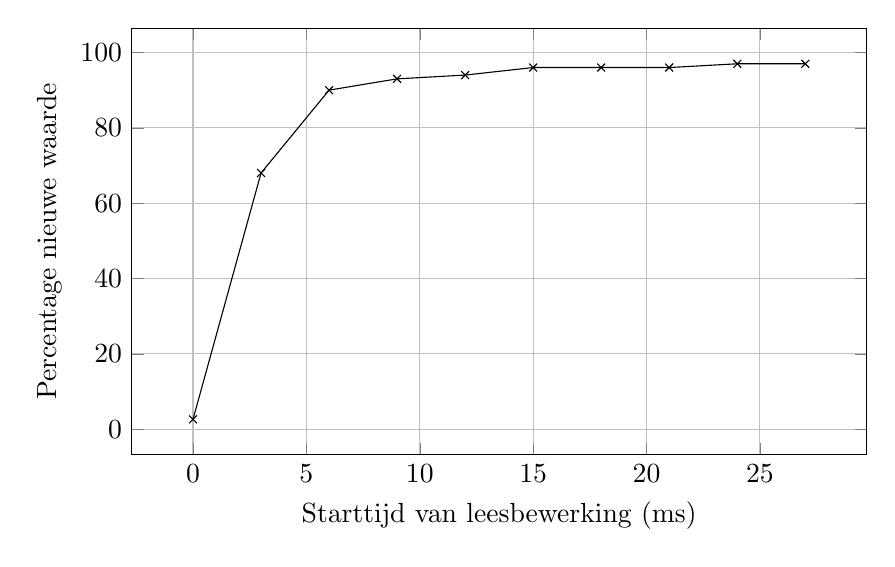
\begin{tikzpicture}
	
	\begin{axis}[
		xlabel={Starttijd van leesbewerking (ms)},
		ylabel={Percentage nieuwe waarde},
		domain = 0:1,
		grid = major,
		height=7cm,
		width=.9\textwidth
	]
	

	\addplot[color=black,mark=x]
	        plot coordinates {
	       		(0, 2.6)
				(3, 68)
				(6,90)
				(9,93)
				(12,94)
				(15,96)
				(18,96)
				(21,96)
				(24,97)
				(27,97)
	        };

	\end{axis}
\end{tikzpicture}
\caption{Consistentie: Percentage van de queries dat op een gegeven tijdstip de juiste data leest voor HBase. Het gemiddelde verschil tussen het starten en stoppen van het lezen op een willekeurig record is ongeveer 6ms, in het geval van hetzelfde record kan dit langer duren door het wachten op de lock. }
\label{fig:consistentie-hbase-correct}
\end{figure}


\begin{figure}[tb!]
	\begin{minipage}{0.5\textwidth} 
	\textbf{Schrijven}
	\begin{enumerate}
	\item Lock de rij(en), om te beschermen tegen gelijktijdige lees- en schrijfacties. 
	\item Haal het huidige schrijfnummer op
	\item Voeg aanpassingen toe aan WAL (Write Ahead Log)
	\item Pas aanpassing toe op de Memstore (cache geheugen)
	\item Commit de transactie, m.a.w. zet het leespunt op het nieuwe schrijfnummer
	\item Unlock de rijen
	\end{enumerate}
	\end{minipage} \hfill
	\begin{minipage}{0.3\textwidth} 
	\textbf{Lezen}
	\begin{enumerate}
	\item Open de lezer
	\item Ga naar het huidige leespunt
	\item Filter al de Key-Value paren met schrijfnummer > leespunt
	\item Sluit de lezer
	\end{enumerate}
	\end{minipage}
	\caption{HBase: Het vereenvoudigde lees- en schrijfmodel voor strikte consistentie in HBase naar Lars Hofhansl\cite{hbase-acid}}\label{fig:consistency-hbase-uitleg}
\end{figure}

\paragraph{MongoDB} MongoDB biedt strikte consistentie aan als er van de primary gelezen wordt maar er zijn ook andere schrijf- en leesmethodes. Een verschil met HBase is dat het bij alle mogelijke lees- en schrijfmethodes mogelijk is om de nieuwe data al te lezen vooraleer de schrijfbewerking beëindigd is. Een schrijfbewerking wacht op de server nog na het schrijven en vrijgeven van zijn schrijf lock. Een verklaring is hiervoor niet gevonden.

Uit figuren \ref{fig:consistentie-mongodb-primary}, \ref{fig:consistentie-mongodb-primarypreferred}, \ref{fig:consistentie-mongodb-secondary}, \ref{fig:consistentie-mongodb-secondarypreferred} en \ref{fig:consistentie-mongodb-nearest} kan een analyse gemaakt worden hoeveel kans er is dat een leesbewerking de nieuwe data al zal lezen. Voor lezer 1 tot 5, dit zijn tijdstippen 0, 2, 4, 6 en 8 ms, is een kans berekend ten opzichte van het starttijdstip. Een grafische voorstelling voor de vier leesconfiguratie bevindt zich in figuur \ref{fig:consistentie-mongodb-correct}. 

Uit figuren \ref{fig:consistentie-mongodb-verschillende-schrijfacties} blijkt dat er geen significant verschil is tussen de leesacties onder verschillende schrijfgaranties, indien men de starttijdstippen vergelijkt. De schrijfconfiguraties geven geen garanties tijdens het uitvoeren maar enkel na de voltooiing van de schrijfoperatie.  

Uit tabel \ref{table:consistentie-mongodb-inconsistency} blijkt dat het in MongoDB niet gegarandeerd is dat als een lezer de nieuwe waarde leest, dat al de overige lezers dat ook zullen doen. In dit geval was het schrijven nog niet voltooid en een bepaalde lezer leest de nieuwe data al. Maar een bewerking die later gestart is, leest de oude waarde nog. Dit kan verklaard worden doordat het verschillende servers zijn waarop gelezen wordt. In dit geval waren het verschillende lezers en dus verschillende gebruikers, maar de MongoDB driver controleert periodiek welke server het dichtste bij is. Dit controle kan tussen deze 2 bewerkingen gebeuren en men kan van een andere instantie lezen (in het geval de leesconfiguratie niet op primary staat). Er is bij MongoDB géén garantie op monotone leesbewerkingen. 

Aangezien er in de testomgeving een uniforme netwerkvertraging is naar alle instanties, volgt de data de veronderstelling dat de dichtstbijzijnde node in iets minder 1/3 van de gevallen een primary is en iets meer dan 2/3 een secondary. Met 5\% afwijking is het moeilijk te stellen dat deze significant is. 

Tenslotte hebben primary en primary-preferred in deze testen geen significante verschillen. Dit komt omdat de primary heel de tijd beschikbaar is. 

\begin{table}
\centering
\begin{tabular}{l | l l l l}
Lezer & Start lezen (ms) & Stop lezen (ms) & Gelezen waarde & Correct? \\
\hline
\multirow{2}{*}{1} & 2,200 & 3,213 & 12553\textbf{3}813315 & Nee\\
 & 13,426 & 14,279 & 12553\textbf{4}813315 & Ja \\
 \multirow{2}{*}{3} & 17,458 & 18,834 & 12553\textbf{3}813315 & Nee\\
 & 29,063 & 29,897 & 12553\textbf{3}813315& Ja \\
\end{tabular}
\caption{Consistentie: Ruwe data van MongoDB test waarbij inconsistente data wordt gelezen na het lezen van consistente data op verschillende lezers met het lezen via nearest en schrijven via fsync\_safe}
\label{table:consistentie-mongodb-inconsistency}
\end{table}


\begin{figure}[!htf]

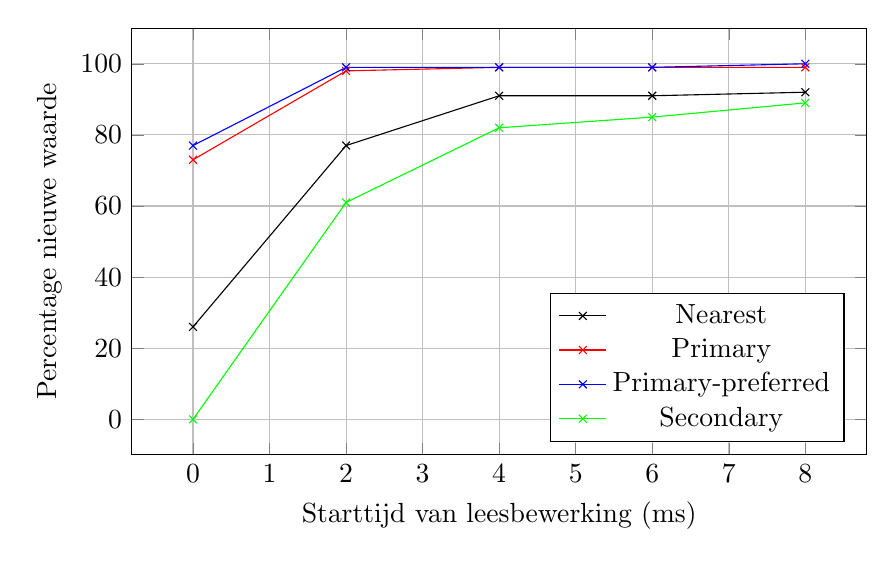
\begin{tikzpicture}
	
	\begin{axis}[
		xlabel={Starttijd van leesbewerking (ms)},
		ylabel={Percentage nieuwe waarde},
		domain = 0:1,
		grid = major,
		height=7cm,
		width=.9\textwidth,
		legend pos= south east
	]
	
	\addplot[color=black,mark=x]
	        plot coordinates {
	       		(0, 26)
				(2, 77)
				(4,91)
				(6,91)
				(8,92)
	        };
	\addlegendentry{Nearest}

	\addplot[color=red,mark=x]
	        plot coordinates {
	       		(0, 73)
				(2, 98)
				(4,99)
				(6,99)
				(8,99)
	        };
	\addlegendentry{Primary}
	
	\addplot[color=blue,mark=x]
      plot coordinates {
	       		(0, 77)
				(2, 99)
				(4,99)
				(6,99)
				(8,100)
      };
	\addlegendentry{Primary-preferred}
	
	\addplot[color=green,mark=x]
   plot coordinates {
	       		(0, 0)
				(2, 61)
				(4,82)
				(6,85)
				(8,89)
   };
	\addlegendentry{Secondary}
	\end{axis}
\end{tikzpicture}
\caption{Consistentie: Percentage van de queries dat van de eerste keer juist de data leest bij 0ms, 2ms, 4ms, 6ms en 8ms voor MongoDB. De gemiddelde vertraging op een onafhankelijke leesoperatie is 1ms. }
\label{fig:consistentie-mongodb-correct}
\end{figure}


\paragraph{Samenvatting} Beide database systemen bieden strikte consistentie aan maar hebben een verschillende uitwerking hiervan: bij HBase worden de leesoperaties uitgesteld tot de volledige voltooiing van de schrijfoperatie, bij MongoDB zal de data al vroeger beschikbaar zijn. Beide systemen zijn \textit{session} consistent, \textit{read-your-own-write} en monotoon consistent, indien er bij MongoDB op een primary wordt gelezen.  

\textit{Session}, \textit{read-your-own-write}, \textit{casual} en \textit{monotonic} consistentie zijn niet gegarandeerd in MongoDB indien er niet gelezen wordt op een primaire. De MongoDB driver kan op ieder moment een andere server kiezen in deze gevallen en kan dus nog oude data lezen. 

Een hypothese is dat bij MongoDB het falen van de primary de consistentie garanties zal beïnvloeden, een nieuwe primary kan verkozen worden. Wanneer geen enkele secondary deze update al heeft ontvangen, zou deze dus verloren gaan. Maar een gebruiker zou de data al van de oude primary gelezen kunnen hebben, in dit geval faalt hier de stikte consistentie. Dit gedrag is wel niet getest en bevestigd. HBase heeft deze situatie niet door de keuze om de leesbewerking te verlengen, een gebruiker dient dus langer te wachten op zijn data. 

\paragraph{Implicatie van de resultaten voor een gebruiker} 

\section{Conclusie}
De drie systemen hebben verschillende aanpak naar beschikbaarheid en consistentie. Pgpool-II is het minst geavanceerd systeem door geen automatisch herstel te ondersteunen, maar door de centrale aanpak van de routernode heeft dit systeem geen netwerk verkeer als het niet wordt gebruikt. 

MongoDB is een systeem dat weinig configureerbaar is naar het gedrag bij het falen van een instantie, daarentegen zijn er een verschillende configuratiemogelijkheid naar het lees- en schrijfgedrag. Enkel als er gelezen wordt van de primary, zal er strikte consistentie zijn. Het is nog onduidelijk welke garanties er zijn bij het falen van een primary. In normale situaties is het mogelijk om de nieuwe data snel te lezen. 

HBase is met behulp van Zookeeper configureerbaar naar het gedrag bij falen van een enkele instantie. De onbeschikbaarheidsperiode kan verkleind of vergroot worden. De consistentiegaranties van HBase zijn strikt voor een enkel record maar dit komt wel voor een prijs: een leesactie wordt uitgesteld indien er een de schrijfactie op dat record uitgevoerd wordt. 
\chapter{Conclusie}


% Indien er bijlagen zijn:
\appendixpage*          % indien gewenst
\appendix
%\chapter{De eerste bijlage}
\label{app:A}
In de bijlagen vindt men de data terug die nuttig kunnen zijn voor de
lezer, maar die niet essentieel zijn om het betoog in de normale tekst te
kunnen volgen. Voorbeelden hiervan zijn bronbestanden,
configuratie-informatie, langdradige wiskundige afleidingen, enz.

In een bijlage kunnen natuurlijk ook verdere onderverdelingen voorkomen,
evenals figuren en referenties\cite{h2g2}.

\section{Meer lorem}
\lipsum[50]

\subsection{Lorem 15--17}
\lipsum[15-17]

\subsection{Lorem 18--19}
\lipsum[18-19]

\section{Lorem 51}
\lipsum[51]

%%% Local Variables: 
%%% mode: latex
%%% TeX-master: "masterproef"
%%% End: 

% ... en zo verder tot
%\chapter{De laatste bijlage}
\label{app:n}
In de bijlagen vindt men de data terug die nuttig kunnen zijn voor de
lezer, maar die niet essentieel zijn om het betoog in de normale tekst te
kunnen volgen. Voorbeelden hiervan zijn bronbestanden,
configuratie-informatie, langdradige wiskundige afleidingen, enz.

\section{Lorem 20-24}
\lipsum[20-24]

\section{Lorem 25-27}
\lipsum[25-27]

%%% Local Variables: 
%%% mode: latex
%%% TeX-master: "masterproef"
%%% End: 


\backmatter
% Na de bijlagen plaatst men nog de bibliografie.
% Je kan de  standaard "abbrv" bibliografiestijl vervangen door een andere.
\printglossary

\printbibliography


\end{document}

%%% Local Variables: 
%%% mode: latex
%%% TeX-master: t
%%% End: 
